\documentclass[10pt]{beamer}

\usetheme[progressbar=frametitle]{metropolis}

\usepackage{booktabs}
\usepackage[scale=2]{ccicons}

\usepackage{pgfplots}
\usepgfplotslibrary{dateplot}

\usepackage{xspace}
\newcommand{\themename}{\textbf{\textsc{metropolis}}\xspace}
 
\usepackage{tikz}
\usetikzlibrary{matrix,chains,positioning,decorations.pathreplacing,arrows}

\usepackage{mathtools}

\title{Patient Similarity}
\subtitle{A textual recommender system and other text mining approaches for clinical data}
\date{\today}
\author{Philipp Hummel}
%\institute{Psiori}
\titlegraphic{\hfill
\includegraphics[height=2.2cm]{logo}}

\begin{document}

\maketitle

\begin{frame}{Idea}
	\begin{itemize}
		\item Doctors write down most important information about the patient in physician letters
		\item Doctors often face unusual patients; therapy decision is unclear
		\item In those cases: retrieve letters of similar patients from database to support clinical decision making
	\end{itemize}
\end{frame}


\begin{frame}[fragile]{Sample Letter}

  
\end{frame}


\begin{frame}{Data Clean-Up}

Two types of duplicates: Exact copies and Follow-Ups

Two approaches for finding them: String Matching and Bag of Words

\bigskip

Bag of Words Example:

$d_{1}=$ ``The patients with disease A.'' \\ $d_{2}=$ ``The patients with disease B.''

\[
\textbf{v}_{d_1}=\begin{array}{c}
1\\
1\\
1\\
0
\end{array}\ \textbf{v}_{d_2}=\begin{array}{c}
1\\
1\\
0\\
1
\end{array}\ \begin{array}{c}
\rm{patient}\\
\rm{disease}\\
\rm{A}\\
\rm{B}\\
\end{array}
\]


\end{frame}

\begin{frame}{Paragraph Extraction}

Rule-based extraction of several paragraphs

Semi-automatic outlier detection

\begin{center}
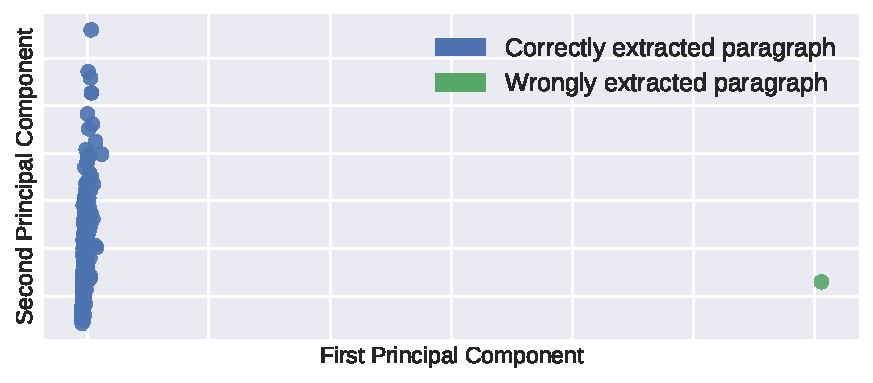
\includegraphics[height=4.2cm]{bow_find_odd}
\end{center}

\end{frame}

\begin{frame}{Paragraph Classification}
	\begin{itemize}
		\item Embed all paragraphs into different vector space models like bag of words, tf-idf, paragraph vector
		\item use these embeddings and hand-made labels as inputs to a classifier
		\item see if classifier can learn to identify different kinds of paragraphs
	\end{itemize}

\begin{center}
	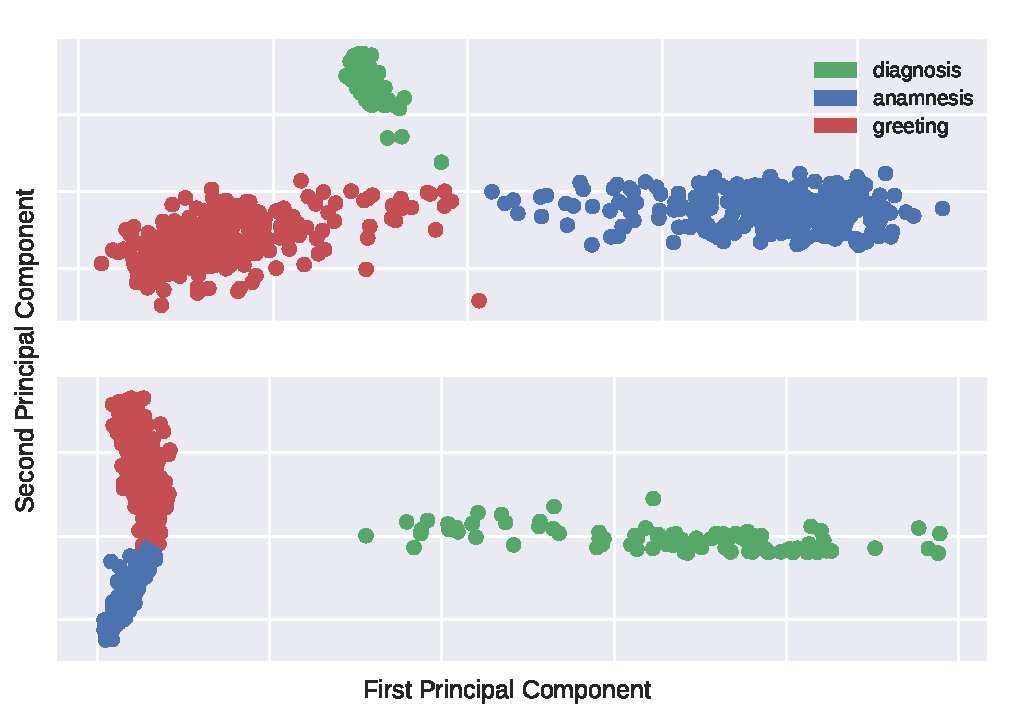
\includegraphics[height=4.6cm]{para2vec_tfidf_pca}
\end{center}	

\end{frame}


\begin{frame}{Recommender System}
	
	\begin{itemize}
		\item Find similar letters based on distance of corresponding vectors in the embedding space
		\item How to find which embedding works best? Supervised Information!
		\item Our Data: Grouping of letters into groups of similars
		\item Our Metric: How often are the similars ranked by algorithm into the top N
		\item tf-idf turns out to be best method; paragraph vector not much worse
	\end{itemize}
	
\end{frame}


\begin{frame}{Experiment}
	
	
\end{frame}


\begin{frame}{Results -- Inter Rater Agreement}
	\begin{itemize}
	\item We measure correlation with spearman rank correlation
	\item Often Expert Ratings are more consistent than student ratings
	\item This is similar in our case
	\item We therefore discard student data for further analysis
	\end{itemize}
\end{frame}


\begin{frame}{Results -- Best vs. Random Letter}
	How much better than chance is our recommendation?
	\begin{center}
		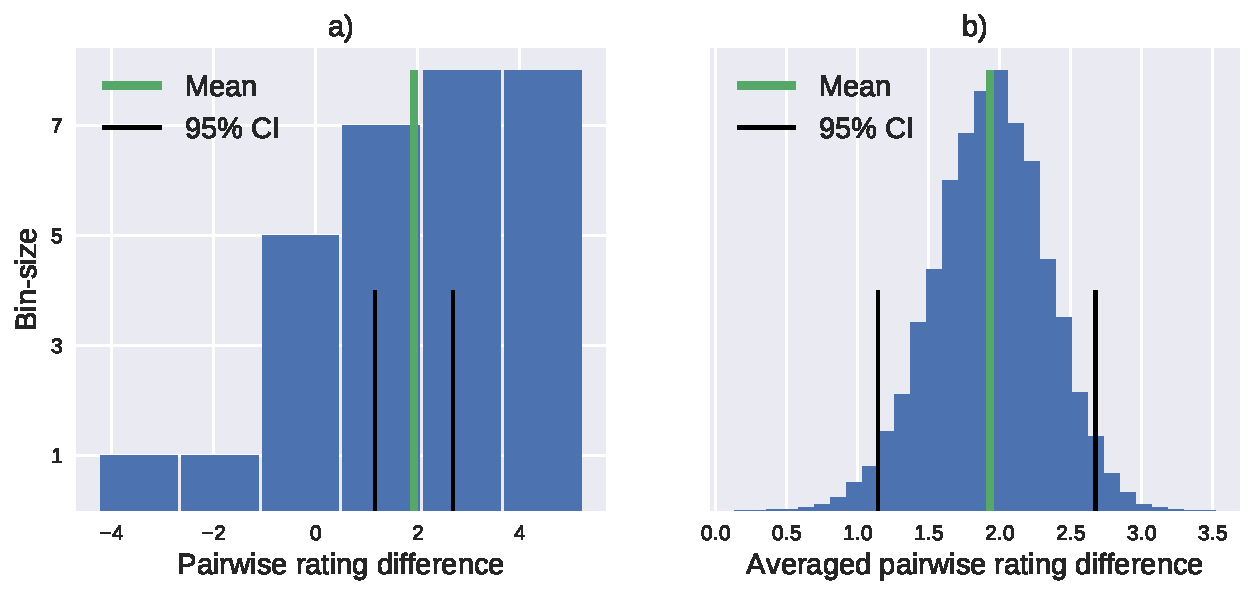
\includegraphics[height=4.8cm]{both_diff_tf}
	\end{center}
\end{frame}


\begin{frame}{Results -- Cosine Similarity and Subject Ratings}
	The recommender system produces a ranking of the letters, but can we use absolute distance (or similarity) information as well?
	
	\begin{center}
		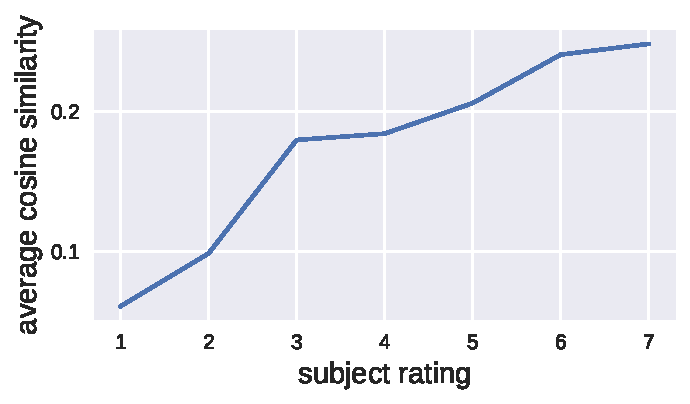
\includegraphics[height=4.2cm]{rating_vs_sim_mean}
	\end{center}
	
\end{frame}


\begin{frame}{Results -- Cosine Similarity and Subject Ratings -- More Details}
	Plot all pairs as data points. Subject rating vs. Cosine Similarity
	\begin{center}
		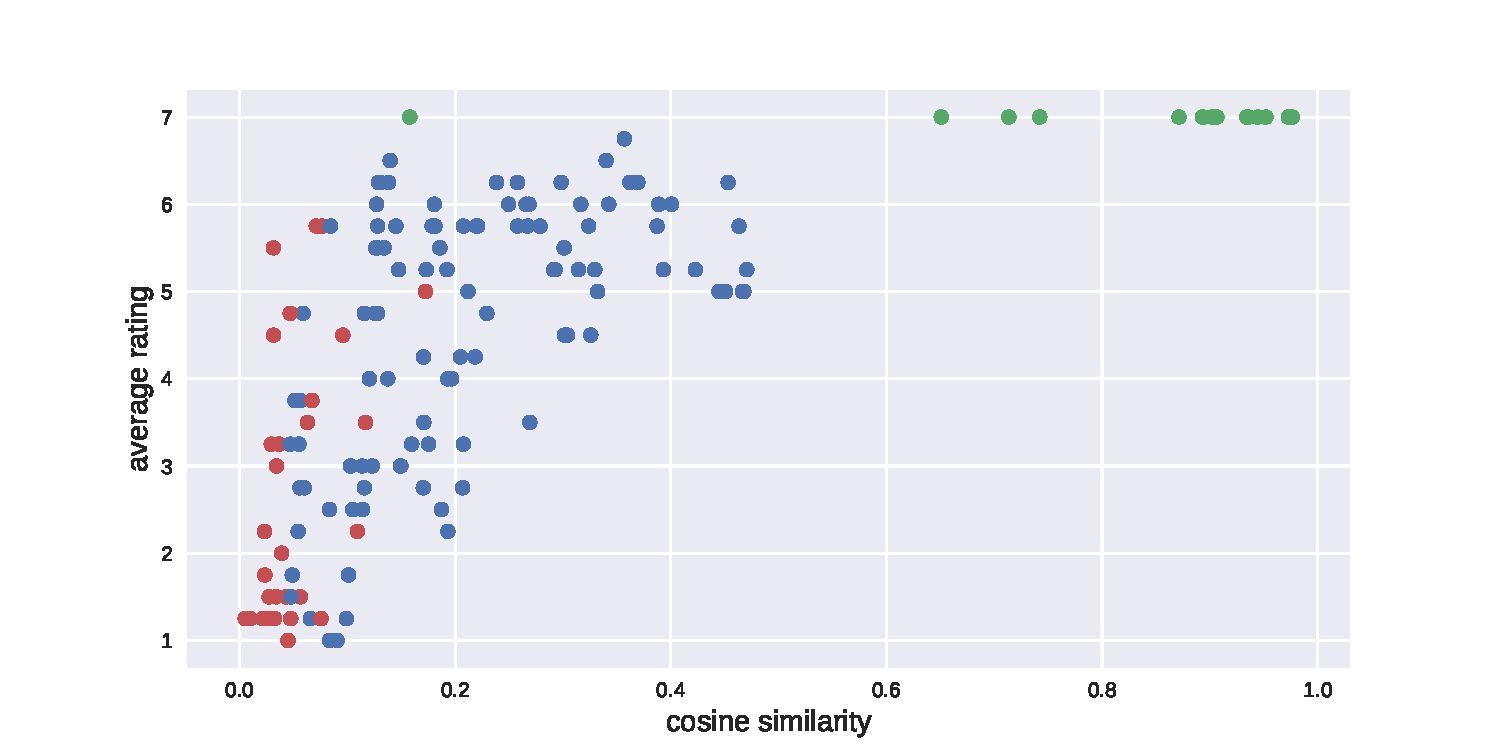
\includegraphics[height=5.2cm]{rating_vs_similarity}
	\end{center}
\end{frame}


\begin{frame}{Results -- Precision and Recall}
	\begin{itemize}
		\item Precision $P(relevant|retrieved)$ is easy to compute
		\item Every letter with rating $>5$ is relevant
		\item We cannot know recall $P(retrieved|relevant)$, because we do not know all relevant letters for a given information need
		\item Recall is not so important for our setting. We do care only whether 5 good letters are retrieved. Not whether all relevant letters are retrieved.
		\item We can still look at the correlation between ranking of algorithm and ranking of subjects. 
	\end{itemize}
\end{frame}


\begin{frame}{Results -- Precision}
	How good is precision in different recommending scenarios?
	\begin{center}
		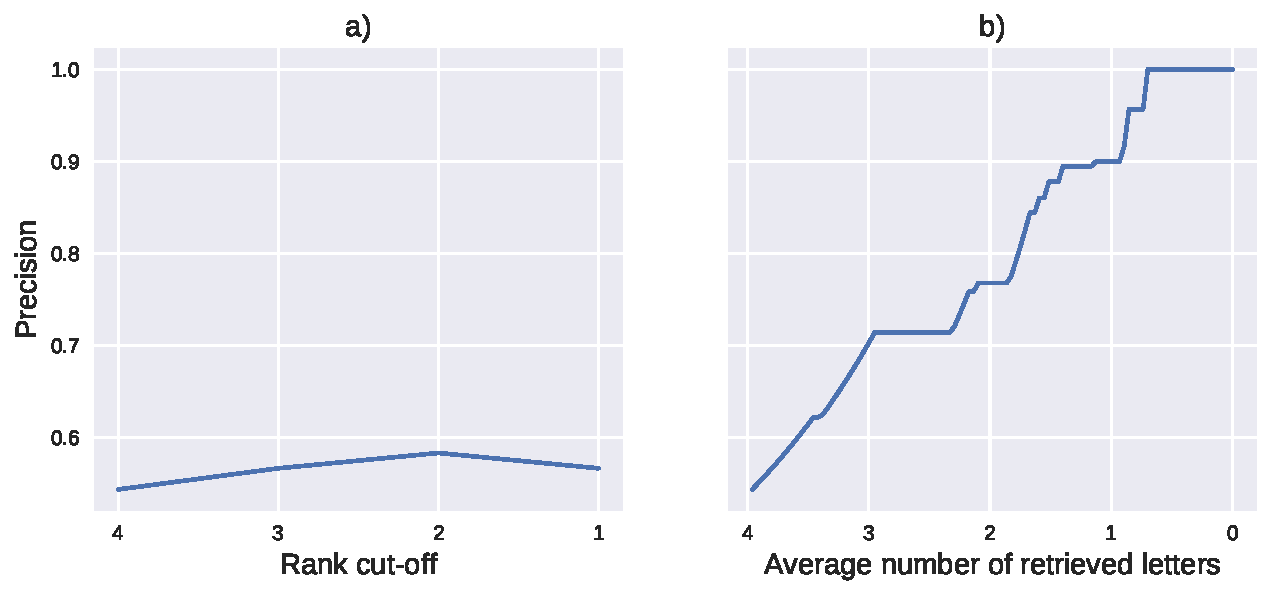
\includegraphics[height=5.2cm]{precision_rank_sim}
	\end{center}
\end{frame}


\begin{frame}{Results -- Recall proxy}
	We can look at correlation between ranking of subjects and ranking of algorithm with spearman rank correlation
	\begin{itemize}
		\item Algo -- Expert Agreement: 0.39
		\item Inter Expert Agreement: 0.72
	\end{itemize}
\end{frame}


\begin{frame}{Considerations of Usability}
	Two reasons why results are probably better in reality than it seems here:
	\begin{itemize}
		\item subjects might adjust their ratings, when all presented examples are bad. Therefore somewhat similar letters might be rated more similar than they really are.
		\item in bigger database we expect more letters with high cosine similarity
	\end{itemize}
\end{frame}


\begin{frame}{Possibilities to improve}
	Can we use the embeddings of two different embedding methods to obtain better results? Paragraph vector seems most promising.
	
	\begin{center}
		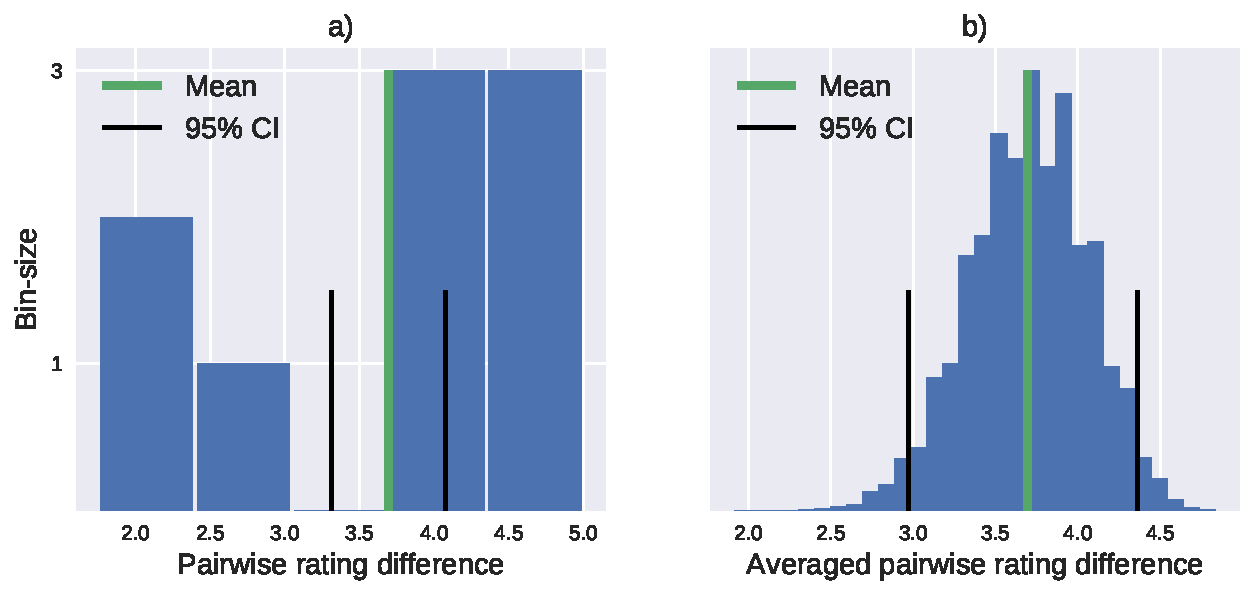
\includegraphics[height=4.9cm]{both_diff_pv}
	\end{center}
\end{frame}


\begin{frame}{Additional Application -- Intelligent Search}
	\begin{itemize}
		\item Say we want to find all letters of patients with a specific feature.
		\item Traditionally: search database with string matching algorithms.
		\item Hardly doable in some cases
		\item Can we do better with embedding methods?
		\item We do experiment to find all letters of patients with a specific disease.
	\end{itemize}

\end{frame}


\begin{frame}{Intelligent Search -- Results}
	For five diseases: How expensive (timewise) is it to find different fractions of the relevant letters?\\
	We start with one letter and look for the next best match first with cosine similarity, then with classifier.
	\begin{center}
		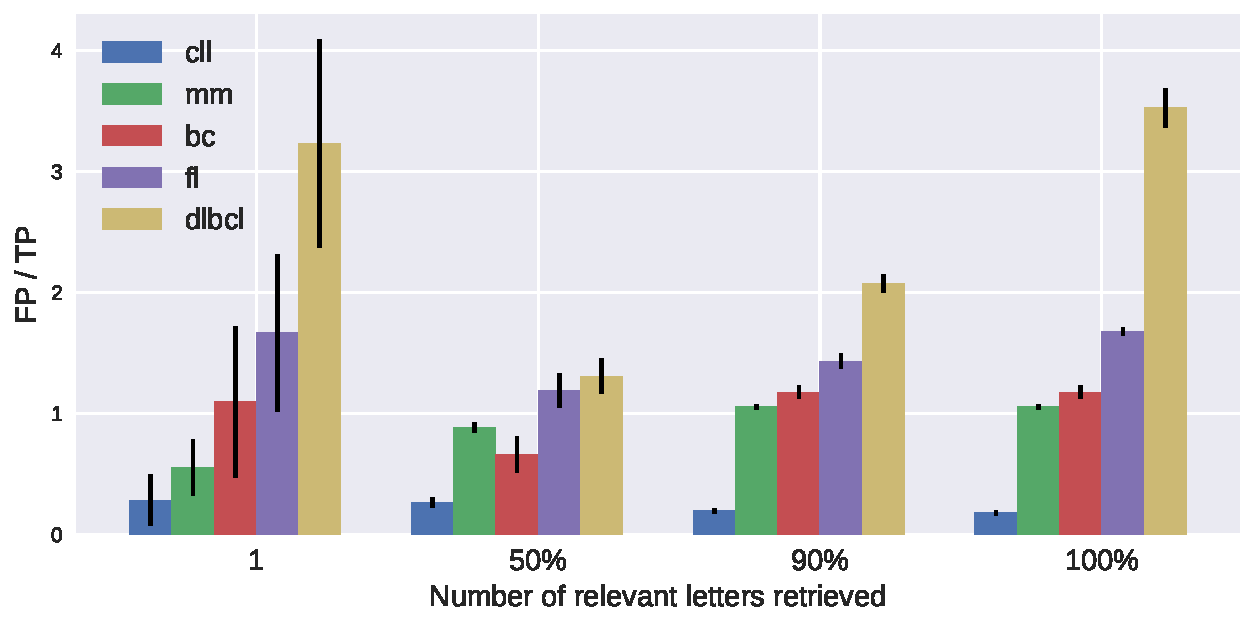
\includegraphics[height=4.9cm]{intelligent_search}
	\end{center}
	Possible application for text mining in law etc.?!
\end{frame}

\begin{frame}[standout]
  Questions?
\end{frame}

\appendix



\end{document}
